% Options for packages loaded elsewhere
\PassOptionsToPackage{unicode}{hyperref}
\PassOptionsToPackage{hyphens}{url}
%
\documentclass[
]{article}
\title{Report with Rmarkdown

Report data analysis with Rmarkdown authoring framework, part 1: Theory}
\author{Thomas Huet, University of Oxford}
\date{January 2022}

\usepackage{amsmath,amssymb}
\usepackage{lmodern}
\usepackage{iftex}
\ifPDFTeX
  \usepackage[T1]{fontenc}
  \usepackage[utf8]{inputenc}
  \usepackage{textcomp} % provide euro and other symbols
\else % if luatex or xetex
  \usepackage{unicode-math}
  \defaultfontfeatures{Scale=MatchLowercase}
  \defaultfontfeatures[\rmfamily]{Ligatures=TeX,Scale=1}
\fi
% Use upquote if available, for straight quotes in verbatim environments
\IfFileExists{upquote.sty}{\usepackage{upquote}}{}
\IfFileExists{microtype.sty}{% use microtype if available
  \usepackage[]{microtype}
  \UseMicrotypeSet[protrusion]{basicmath} % disable protrusion for tt fonts
}{}
\makeatletter
\@ifundefined{KOMAClassName}{% if non-KOMA class
  \IfFileExists{parskip.sty}{%
    \usepackage{parskip}
  }{% else
    \setlength{\parindent}{0pt}
    \setlength{\parskip}{6pt plus 2pt minus 1pt}}
}{% if KOMA class
  \KOMAoptions{parskip=half}}
\makeatother
\usepackage{xcolor}
\IfFileExists{xurl.sty}{\usepackage{xurl}}{} % add URL line breaks if available
\IfFileExists{bookmark.sty}{\usepackage{bookmark}}{\usepackage{hyperref}}
\hypersetup{
  pdfauthor={Thomas Huet, University of Oxford},
  hidelinks,
  pdfcreator={LaTeX via pandoc}}
\urlstyle{same} % disable monospaced font for URLs
\usepackage[margin=1in]{geometry}
\usepackage{color}
\usepackage{fancyvrb}
\newcommand{\VerbBar}{|}
\newcommand{\VERB}{\Verb[commandchars=\\\{\}]}
\DefineVerbatimEnvironment{Highlighting}{Verbatim}{commandchars=\\\{\}}
% Add ',fontsize=\small' for more characters per line
\usepackage{framed}
\definecolor{shadecolor}{RGB}{248,248,248}
\newenvironment{Shaded}{\begin{snugshade}}{\end{snugshade}}
\newcommand{\AlertTok}[1]{\textcolor[rgb]{0.94,0.16,0.16}{#1}}
\newcommand{\AnnotationTok}[1]{\textcolor[rgb]{0.56,0.35,0.01}{\textbf{\textit{#1}}}}
\newcommand{\AttributeTok}[1]{\textcolor[rgb]{0.77,0.63,0.00}{#1}}
\newcommand{\BaseNTok}[1]{\textcolor[rgb]{0.00,0.00,0.81}{#1}}
\newcommand{\BuiltInTok}[1]{#1}
\newcommand{\CharTok}[1]{\textcolor[rgb]{0.31,0.60,0.02}{#1}}
\newcommand{\CommentTok}[1]{\textcolor[rgb]{0.56,0.35,0.01}{\textit{#1}}}
\newcommand{\CommentVarTok}[1]{\textcolor[rgb]{0.56,0.35,0.01}{\textbf{\textit{#1}}}}
\newcommand{\ConstantTok}[1]{\textcolor[rgb]{0.00,0.00,0.00}{#1}}
\newcommand{\ControlFlowTok}[1]{\textcolor[rgb]{0.13,0.29,0.53}{\textbf{#1}}}
\newcommand{\DataTypeTok}[1]{\textcolor[rgb]{0.13,0.29,0.53}{#1}}
\newcommand{\DecValTok}[1]{\textcolor[rgb]{0.00,0.00,0.81}{#1}}
\newcommand{\DocumentationTok}[1]{\textcolor[rgb]{0.56,0.35,0.01}{\textbf{\textit{#1}}}}
\newcommand{\ErrorTok}[1]{\textcolor[rgb]{0.64,0.00,0.00}{\textbf{#1}}}
\newcommand{\ExtensionTok}[1]{#1}
\newcommand{\FloatTok}[1]{\textcolor[rgb]{0.00,0.00,0.81}{#1}}
\newcommand{\FunctionTok}[1]{\textcolor[rgb]{0.00,0.00,0.00}{#1}}
\newcommand{\ImportTok}[1]{#1}
\newcommand{\InformationTok}[1]{\textcolor[rgb]{0.56,0.35,0.01}{\textbf{\textit{#1}}}}
\newcommand{\KeywordTok}[1]{\textcolor[rgb]{0.13,0.29,0.53}{\textbf{#1}}}
\newcommand{\NormalTok}[1]{#1}
\newcommand{\OperatorTok}[1]{\textcolor[rgb]{0.81,0.36,0.00}{\textbf{#1}}}
\newcommand{\OtherTok}[1]{\textcolor[rgb]{0.56,0.35,0.01}{#1}}
\newcommand{\PreprocessorTok}[1]{\textcolor[rgb]{0.56,0.35,0.01}{\textit{#1}}}
\newcommand{\RegionMarkerTok}[1]{#1}
\newcommand{\SpecialCharTok}[1]{\textcolor[rgb]{0.00,0.00,0.00}{#1}}
\newcommand{\SpecialStringTok}[1]{\textcolor[rgb]{0.31,0.60,0.02}{#1}}
\newcommand{\StringTok}[1]{\textcolor[rgb]{0.31,0.60,0.02}{#1}}
\newcommand{\VariableTok}[1]{\textcolor[rgb]{0.00,0.00,0.00}{#1}}
\newcommand{\VerbatimStringTok}[1]{\textcolor[rgb]{0.31,0.60,0.02}{#1}}
\newcommand{\WarningTok}[1]{\textcolor[rgb]{0.56,0.35,0.01}{\textbf{\textit{#1}}}}
\usepackage{longtable,booktabs,array}
\usepackage{calc} % for calculating minipage widths
% Correct order of tables after \paragraph or \subparagraph
\usepackage{etoolbox}
\makeatletter
\patchcmd\longtable{\par}{\if@noskipsec\mbox{}\fi\par}{}{}
\makeatother
% Allow footnotes in longtable head/foot
\IfFileExists{footnotehyper.sty}{\usepackage{footnotehyper}}{\usepackage{footnote}}
\makesavenoteenv{longtable}
\usepackage{graphicx}
\makeatletter
\def\maxwidth{\ifdim\Gin@nat@width>\linewidth\linewidth\else\Gin@nat@width\fi}
\def\maxheight{\ifdim\Gin@nat@height>\textheight\textheight\else\Gin@nat@height\fi}
\makeatother
% Scale images if necessary, so that they will not overflow the page
% margins by default, and it is still possible to overwrite the defaults
% using explicit options in \includegraphics[width, height, ...]{}
\setkeys{Gin}{width=\maxwidth,height=\maxheight,keepaspectratio}
% Set default figure placement to htbp
\makeatletter
\def\fps@figure{htbp}
\makeatother
\setlength{\emergencystretch}{3em} % prevent overfull lines
\providecommand{\tightlist}{%
  \setlength{\itemsep}{0pt}\setlength{\parskip}{0pt}}
\setcounter{secnumdepth}{-\maxdimen} % remove section numbering
\newlength{\cslhangindent}
\setlength{\cslhangindent}{1.5em}
\newlength{\csllabelwidth}
\setlength{\csllabelwidth}{3em}
\newlength{\cslentryspacingunit} % times entry-spacing
\setlength{\cslentryspacingunit}{\parskip}
\newenvironment{CSLReferences}[2] % #1 hanging-ident, #2 entry spacing
 {% don't indent paragraphs
  \setlength{\parindent}{0pt}
  % turn on hanging indent if param 1 is 1
  \ifodd #1
  \let\oldpar\par
  \def\par{\hangindent=\cslhangindent\oldpar}
  \fi
  % set entry spacing
  \setlength{\parskip}{#2\cslentryspacingunit}
 }%
 {}
\usepackage{calc}
\newcommand{\CSLBlock}[1]{#1\hfill\break}
\newcommand{\CSLLeftMargin}[1]{\parbox[t]{\csllabelwidth}{#1}}
\newcommand{\CSLRightInline}[1]{\parbox[t]{\linewidth - \csllabelwidth}{#1}\break}
\newcommand{\CSLIndent}[1]{\hspace{\cslhangindent}#1}
\ifLuaTeX
  \usepackage{selnolig}  % disable illegal ligatures
\fi

\begin{document}
\maketitle

{
\setcounter{tocdepth}{2}
\tableofcontents
}
\begin{figure}
\centering

\includegraphics[width=5.20833in,height=\textheight]{www/logo.png}
\caption{1. Report with R Markdown - Theory}
\end{figure}

\hypertarget{authoring-framework-10-min}{%
\section{Authoring framework (10
min)}\label{authoring-framework-10-min}}

R Markdown is an authoring framework for data science. It permits to
create a computational -- or data-driven -- document, with a notebook
interface for report generation. R Markdown combines:

\begin{itemize}
\item
  a YAML header for the document metadata
\item
  many code chunks (R code) for the logics
\item
  many narrative parts (Markdown syntax)
\end{itemize}

YAML{~header}

narrative text

{R code}

narrative text

{R code}

{\ldots{}}

{\ldots{}}

\hypertarget{r-markdown-30-min}{%
\section{R Markdown (30 min)}\label{r-markdown-30-min}}

On the creation of a new R Markdown document, the only package required
is \{\texttt{knitr}\}. Knitr package is designed to be a
`\emph{transparent engine for dynamic report generation with R}' (Xie
(2022))

\hypertarget{document-creation}{%
\subsection{Document creation}\label{document-creation}}

In \href{https://rmarkdown.rstudio.com/}{RStudio}:
 \texttt{File\ \textgreater{}\ New\ file\ \textgreater{}\ R\ Markdown...}
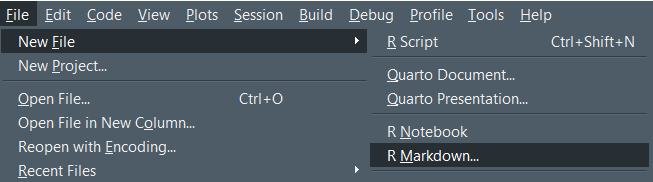
\includegraphics[width=6.25in,height=\textheight]{https://raw.githubusercontent.com/zoometh/oxford/main/R4A/www/rmd_create.png}

The parameters (\texttt{Title}, \texttt{Author}) can be changed later on
the \protect\hyperlink{yaml}{YAML header}


\includegraphics[width=6.25in,height=\textheight]{https://raw.githubusercontent.com/zoometh/oxford/main/R4A/www/rmd_create_rmd.png}

A new tab is created:

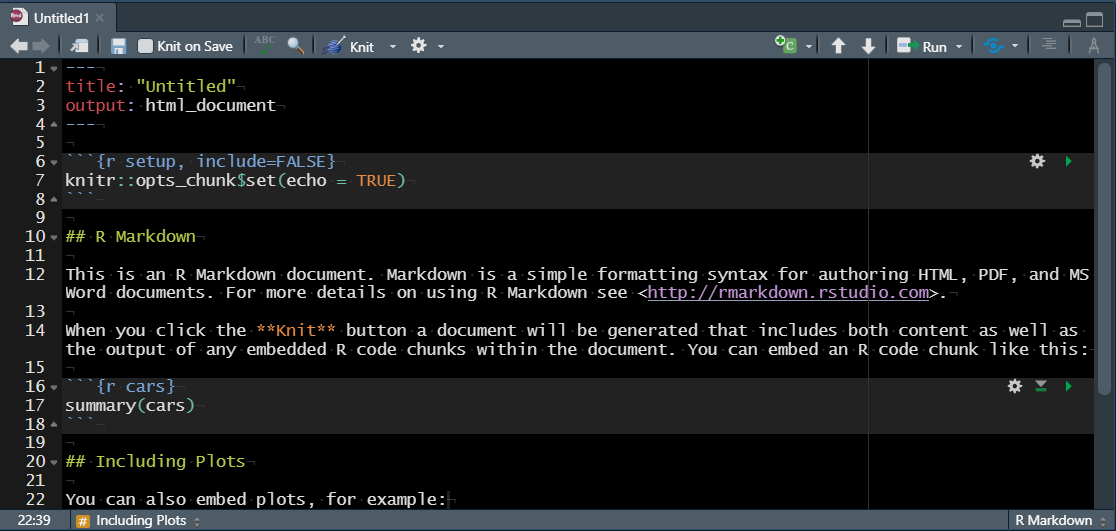
\includegraphics[width=6.25in,height=\textheight]{https://raw.githubusercontent.com/zoometh/oxford/main/R4A/www/rmd_create_rmd_new.png}

\hypertarget{navigate}{%
\subsubsection{Navigate}\label{navigate}}

Use \href{https://rmarkdown.rstudio.com/}{RStudio} GUI tools

\begin{itemize}
\item
    knit when save the document
\item
    check spelling
\item
    knit the document
\item
    run \href{https://rstudio.github.io/visual-markdown-editing/}{Visual
  R Markdown}\\
  -  new editing tools
\item
    create a new code chunk (R, Bash, D3, Python, etc.)
\item
    run a part or the whole document
\item
    publish the document
\item
    run \href{https://rstudio.github.io/visual-markdown-editing/}{Visual
  R Markdown}
\end{itemize}

\hypertarget{environment}{%
\subsection{Environment}\label{environment}}

R Markdown use Markdown syntax, supports HTML tags, BibTex bibliographic
references, 3D objects

\hypertarget{markdown-syntax}{%
\subsubsection{Markdown syntax}\label{markdown-syntax}}

\textbf{Markdown syntax} is used by different code-oriented frameworks:

\begin{itemize}
\tightlist
\item
  \href{https://hub.mybinder.turing.ac.uk/user/ipython-ipython-in-depth-qd7itkd2/notebooks/binder/Index.ipynb}{Jupyter}
\item
  \href{https://github.com/zoometh/oxford/tree/main/R4Archaeologists\#rmarkdown}{GitHub}
\item
  \href{https://sketchfab.com/3d-models/roche-de-larcher-a5c0771d898d4816950570cd7fb1be37}{Sketchfab}
\item
  \href{https://eamena.slack.com/archives/D02KMQULWVD/p1637257246040200}{Slack}
\item
  \href{https://martinhinz.github.io/smada2021/book/preface.html}{bookdown}
\item
  \href{https://stackoverflow.com/a/14747656/2854081}{Stackoverflow}
\item
  etc.
\end{itemize}

Markdown syntax is an \textbf{easy-to-write plain text} syntax

\hypertarget{styling}{%
\paragraph{Styling}\label{styling}}

\begin{longtable}[]{@{}ll@{}}
\toprule
code in R Markdown & Output \\
\midrule
\endhead
\texttt{**bold**,\ \_\_bold\_\_} & \textbf{bold}, \textbf{bold} \\
\texttt{*italic*,\ \_italic\_} & \emph{italic}, \emph{italic} \\
\texttt{code} & \texttt{code} \\
\texttt{hyphen\ -\/-\ inserted\ -\/-\ in\ a\ sentence} & hyphen --
inserted -- in a sentence \\
\texttt{H\textasciitilde{}2\textasciitilde{}O} & H\textsubscript{2}O \\
\texttt{10\^{}−19\^{}} & 10\textsuperscript{−19} \\
\texttt{\$\$\textbackslash{}sum\_\{i=1\}\^{}\{n\}\ X\^{}3\_i\$\$} &
\(\sum_{i=1}^{n} X^3_i\) \\
\ldots{} & \ldots{} \\
\bottomrule
\end{longtable}

\begin{itemize}
\tightlist
\item
  comments \texttt{\textgreater{}}
\end{itemize}

\begin{quote}
I am commented
\end{quote}

\begin{itemize}
\tightlist
\item
  line separator
\end{itemize}

\texttt{text\ between\ two\ lines\ -\/-\/-}

\begin{center}\rule{0.5\linewidth}{0.5pt}\end{center}

\hypertarget{hyperlinks-and-bookmarks}{%
\subparagraph{hyperlinks and bookmarks}\label{hyperlinks-and-bookmarks}}

\begin{itemize}
\tightlist
\item
  hyperlinks

  \begin{itemize}
  \item
    Report with R Markdown, part 2:
    \href{https://zoometh.github.io/oxford/R4A/2_R\%20Markdown_Practice}{Practice}
  \item
    \href{https://www.unipi.it/index.php/humanities/item/16574-r4rchaeologists}{
\includegraphics[width=0.52083in,height=\textheight]{www/logo.png}}
  \end{itemize}
\item
  \protect\hyperlink{practice}{bookmarks}
\end{itemize}

\hypertarget{lists}{%
\subparagraph{Lists}\label{lists}}

\begin{itemize}
\item
  numbered

  \begin{enumerate}
  \def\labelenumi{\arabic{enumi}.}
  \tightlist
  \item
    first element
  \item
    second element
  \item
    third element
  \end{enumerate}
\item
  bullet

  \begin{itemize}
  \tightlist
  \item
    first element
  \item
    second element
  \item
    third element

    \begin{itemize}
    \tightlist
    \item
      third element - sub 1
    \item
      third element - sub 2

      \begin{itemize}
      \tightlist
      \item
        third element - sub 2 - subsub 1
      \item
        third element - sub 2 - subsub 2
      \end{itemize}
    \end{itemize}
  \end{itemize}
\end{itemize}

\hypertarget{tables}{%
\subparagraph{Tables}\label{tables}}

\begin{itemize}
\tightlist
\item
  simple table
\end{itemize}

\begin{verbatim}
| Syntax | Description |
| --- | ----------- |
| Header | Title |
| Paragraph | Text |
\end{verbatim}

and

\begin{verbatim}
| Syntax      | Description |
| ----------- | ----------- |
| Header      | Title       |
| Paragraph   | Text        |
\end{verbatim}

produce the same result:

\begin{longtable}[]{@{}ll@{}}
\toprule
Syntax & Description \\
\midrule
\endhead
Header & Title \\
Paragraph & Text \\
\bottomrule
\end{longtable}

\begin{itemize}
\tightlist
\item
  alignements
\end{itemize}

\begin{longtable}[]{@{}lcr@{}}
\toprule
Syntax & Description & Test Text \\
\midrule
\endhead
Header & Title & Here's this \\
Paragraph & Text & And more \\
\bottomrule
\end{longtable}

\hypertarget{footnotes}{%
\subparagraph{Footnotes}\label{footnotes}}

A simple footnote,\footnote{This is the first footnote.} or a longer
one.\footnote{Here's one with multiple paragraphs and code.

  Indent paragraphs to include them in the footnote.

  \texttt{\{\ my\ code\ \}}

  Add as many paragraphs as you like.}

\hypertarget{referring-to-features}{%
\subparagraph{Referring to features}\label{referring-to-features}}

Refer to a R variable (inline R code), code chunk, figure (table,
graphic), etc.

\begin{Shaded}
\begin{Highlighting}[]
\FunctionTok{library}\NormalTok{(archdata)}
\FunctionTok{data}\NormalTok{(}\StringTok{"Handaxes"}\NormalTok{)}
\NormalTok{number.of.axes }\OtherTok{\textless{}{-}} \FunctionTok{nrow}\NormalTok{(Handaxes)}
\FunctionTok{summary}\NormalTok{(Handaxes)}
\end{Highlighting}
\end{Shaded}

\begin{verbatim}
##    Catalog                L               L1               B         
##  Length:600         Min.   : 69.0   Min.   : 15.00   Min.   : 34.00  
##  Class :character   1st Qu.:103.0   1st Qu.: 32.00   1st Qu.: 61.00  
##  Mode  :character   Median :118.0   Median : 39.00   Median : 70.00  
##                     Mean   :121.9   Mean   : 41.64   Mean   : 70.86  
##                     3rd Qu.:136.0   3rd Qu.: 49.00   3rd Qu.: 80.00  
##                     Max.   :242.0   Max.   :136.00   Max.   :123.00  
##        B1               B2               T               T1       
##  Min.   : 18.00   Min.   : 21.00   Min.   :20.00   Min.   : 7.00  
##  1st Qu.: 32.75   1st Qu.: 52.00   1st Qu.:32.00   1st Qu.:13.00  
##  Median : 40.00   Median : 62.00   Median :38.00   Median :16.00  
##  Mean   : 42.21   Mean   : 61.97   Mean   :38.44   Mean   :16.53  
##  3rd Qu.: 50.00   3rd Qu.: 70.00   3rd Qu.:44.00   3rd Qu.:19.00  
##  Max.   :103.00   Max.   :102.00   Max.   :69.00   Max.   :35.00
\end{verbatim}

\begin{itemize}
\tightlist
\item
  variable:
\end{itemize}

`(\ldots) the Furze Platt dataset counts 600 described by 8. The maximal
length (L = 242) (\ldots)'

\begin{itemize}
\item
  chunk
\item
  figure
\item
  bibliographical reference (Hinz (2021))
\end{itemize}

`(\ldots) Dale (2021) (\ldots)' or `(\ldots) studied by Luke Dale (-Dale
(2021)) (\ldots)' or `(\ldots) (see Dale 2021) (\ldots)'

\hypertarget{pararaphs}{%
\subparagraph{Pararaphs}\label{pararaphs}}

\begin{itemize}
\tightlist
\item
  end of line (= \texttt{\textless{}br\textgreater{}} in HTML) with 2 or
  more spaces and return, for example:
\end{itemize}

`Reconnais-toi\\
Cette adorable personne c'est toi\\
Sous le grand chapeau canotier\\
Oeil Nez\\
Ta Bouche\\
Voici l'ovale de ta figure\\
Ton cou Exquis' (Apollinaire, 1913)


\includegraphics[width=6.25in,height=\textheight]{https://raw.githubusercontent.com/zoometh/oxford/main/R4A/www/rmd_eol.png}

\begin{itemize}
\tightlist
\item
  extra spaces (HTML tags)

  \begin{itemize}
  \tightlist
  \item
      \texttt{\&emsp;} means 4 spaces (= a tabulation)
  \item
      \texttt{\&ensp;} means 2 spaces
  \item
    ~ \texttt{\&nbsp;} means 1 space
  \end{itemize}
\end{itemize}

\hypertarget{html}{%
\subsubsection{HTML}\label{html}}

\begin{longtable}[]{@{}ll@{}}
\toprule
code in R Markdown (= HTML) & Output \\
\midrule
\endhead
\texttt{\textless{}span\ style=\textquotesingle{}font-size:\ 30px\textquotesingle{}\textgreater{}Big\ font\textless{}/span\textgreater{}}
& {Big font} \\
\texttt{\textless{}b\textgreater{}bolded\textless{}/b\textgreater{}} &
bolded \\
\texttt{\textless{}span\ style="color:red"\textgreater{}color\textless{}/span\textgreater{}}
& {color} \\
\ldots{} & \ldots{} \\
\bottomrule
\end{longtable}

\hypertarget{bibliographic-references}{%
\subsubsection{Bibliographic
references}\label{bibliographic-references}}

\begin{itemize}
\tightlist
\item
  file \texttt{.bib}
\end{itemize}

\begin{itemize}
\tightlist
\item
  citation in text
\end{itemize}

\begin{longtable}[]{@{}
  >{\raggedright\arraybackslash}p{(\columnwidth - 2\tabcolsep) * \real{0.50}}
  >{\raggedright\arraybackslash}p{(\columnwidth - 2\tabcolsep) * \real{0.50}}@{}}
\toprule
\begin{minipage}[b]{\linewidth}\raggedright
code in R Markdown
\end{minipage} & \begin{minipage}[b]{\linewidth}\raggedright
Output
\end{minipage} \\
\midrule
\endhead
\texttt{@Xie22} & Xie (2022) \\
\texttt{{[}@Xie22{]}} & (Xie 2022) \\
\texttt{{[}credits:\ @Xie22{]}} & (credits: Xie 2022) \\
\texttt{published\ by\ Yihui\ Xie\ {[}-@Xie20;\ -@Xie22{]}} & published
by Yihui Xie (2020; 2022) \\
\ldots{} & \ldots{} \\
\bottomrule
\end{longtable}

\href{https://bookdown.org/yihui/rmarkdown-cookbook/bibliography.html\#bibliography}{
\includegraphics[width=0.20833in,height=\textheight]{www/info_darkblue.png}} 
Bibliographies and citations (Xie, Dervieux, and Riederer 2020)

\hypertarget{d-objects}{%
\subsubsection{3D objects}\label{d-objects}}

\begin{verbatim}
## Warning in snapshot3d(scene = x, width = width, height = height): webshot = TRUE
## requires the webshot2 package; using rgl.snapshot() instead
\end{verbatim}

\begin{figure}

{\centering \includegraphics[width=0.25\linewidth]{C:\Users\THOMAS~1\AppData\Local\Temp\Rtmp8KRghI\file122031105a67} 

}

\caption{iris}\label{fig:unnamed-chunk-2}
\end{figure}

\href{https://www.r-graph-gallery.com/3d_scatter_plot.html}{
\includegraphics[width=0.20833in,height=\textheight]{www/info_darkblue.png}} 
3d scatterplot with R

\hypertarget{export}{%
\subsection{Export}\label{export}}

Export R Markdown in:

\begin{itemize}
\tightlist
\item
  HTML

  \begin{itemize}
  \tightlist
  \item
    this R Markdown document/webpage
  \end{itemize}
\item
  PDF
\item
  LaTex
\item
  etc.
\end{itemize}

Convert

\begin{itemize}
\tightlist
\item
  \href{https://wordtohtml.net/}{Word to HTML online}
\end{itemize}

\hypertarget{writing}{%
\subsection{Writing}\label{writing}}

\hypertarget{r-markdown-structure}{%
\subsubsection{R Markdown structure}\label{r-markdown-structure}}

\hypertarget{code-chunks}{%
\paragraph{Code chunks}\label{code-chunks}}

\begin{itemize}
\tightlist
\item
  header

  \begin{itemize}
  \tightlist
  \item
    include
  \item
    echo
  \item
    eval
  \item
    caption
  \item
    etc.
  \end{itemize}
\item
  body

  \begin{itemize}
  \tightlist
  \item
    R code
  \end{itemize}
\end{itemize}

\hypertarget{yaml}{%
\paragraph{YAML header}\label{yaml}}

Metadata and document configuration

\begin{itemize}
\item
  \texttt{title}: Title
\item
  \texttt{author}: Author
\item
  \texttt{date}:

  \begin{itemize}
  \tightlist
  \item
    ``01/29/22''
  \item
    ``29 January 2022''
  \item
    etc.
  \end{itemize}
\item
  \texttt{toc}: table of contents
\item
  \texttt{bibliography}: bibliographical references
\end{itemize}

\hypertarget{publishing}{%
\subsection{Publishing}\label{publishing}}

\hypertarget{formats}{%
\subsubsection{Formats}\label{formats}}

\begin{itemize}
\item
  PDF
\item
  HTML
\item
  etc.
\end{itemize}

\hypertarget{platforms}{%
\subsubsection{Platforms}\label{platforms}}

\begin{itemize}
\item
  Rpubs
\item
  GitHub/GitLab
\end{itemize}

\hypertarget{practice}{%
\section{Practice (120 min)}\label{practice}}

see \url{https://zoometh.github.io/oxford/R4A/2_Rmarkdown_Practice}

\hypertarget{references}{%
\section*{References}\label{references}}
\addcontentsline{toc}{section}{References}

\hypertarget{refs}{}
\begin{CSLReferences}{1}{0}
\leavevmode\vadjust pre{\hypertarget{ref-Dale21}{}}%
Dale, Luke. 2021. {``An Analysis of the Furze Platt Handaxes at the
Royal Ontario Museum, Toronto.''} \emph{Lithics--The Journal of the
Lithic Studies Society}, no. 40: 65.
\url{http://journal.lithics.org/wp-content/uploads/2021/04/Lithics_40_4_Dale.pdf}.

\leavevmode\vadjust pre{\hypertarget{ref-Hinz21}{}}%
Hinz, Martin. 2021. \emph{Statistical Methods for Archaeological Data
Analysis i: Basic Methods}. Institut für Archäologische Wissenschaften,
Universität Bern.
\url{https://martinhinz.github.io/smada2021/book/preface.html}.

\leavevmode\vadjust pre{\hypertarget{ref-Xie22}{}}%
Xie, Yihui. 2022. {``Knitr. Elegant, Flexible, and Fast Dynamic Report
Generation with r.''} \url{https://yihui.org/knitr/}.

\leavevmode\vadjust pre{\hypertarget{ref-Xie20}{}}%
Xie, Yihui, Christophe Dervieux, and Emily Riederer. 2020. \emph{R
Markdown Cookbook}. Chapman; Hall/CRC.
\url{https://bookdown.org/yihui/rmarkdown-cookbook/}.

\end{CSLReferences}

\end{document}
